\chapter{Related Work}
\label{chap:related_work}
Bitcoin was the first application of a blockchain, and is based on a proof-of-work system to represent a majority decision. The miners collect pending transactions in the network and form potential blocks, illustrated in Figure \ref{fig:blockchain}, and then, hash the contents of this block with an variable nonce to meet a certain criteria~\cite{bitcoin2008}. For Bitcoin this criteria is that the hash must begin with a certain number of zeros, and this number of zeros can be increased or decreased to compensate for variable computational power in the network~\cite{bitcoin2008}. The complexity is varied to maintain around one block per 10 minutes, but the nature of the psudorandomization of hashing algorithms it can be solved in seconds, but it can also take in excess of 20 minutes~\cite{blockchain_info}. As long as the majority of computational power is controlled by nodes not trying to attack the network, the blockchain serves as a ledger of witnessed transactions with proved ownership.

\begin{figure}[h]
    \centering
    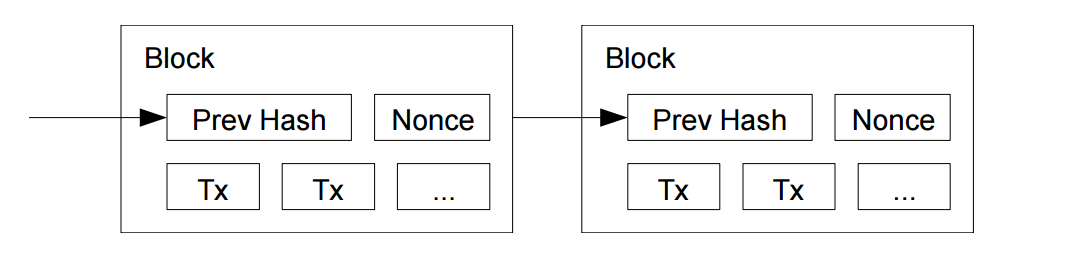
\includegraphics[width=1\textwidth]{blockchain}
    \caption{Visualization of blockchain \cite{bitcoin2008}}
    \label{fig:blockchain}
\end{figure}

The growing success of crypto-currency, with Bitcoin above half the total market cap~\cite{coinmarketcap}, the incentive for miners has increased with the price. \cite{VRANKEN20171} estimates the total power consumption to be between 100 and 500 MW, the equivalent of a small nation state, and the inefficiency of the Proof-of-Work (PoW) has made Proof-of-Stake (PoS) look like a strong candidate. In the later years, several PoS currencies has been proposed and launched~\cite{Li2017,nxt_whitepaper,blackcoin_pos} but have yet to achieve large market adoption. The PoS scheme maintain consensus in the network based on the nodes stake, and the consensus is fast and uses negligible resources. PoS implementations sill suffer from some major security concerns, and proposed attacks like \textit{nothing at stake} and \textit{long-range attacks} is probably holding the adoption back~\cite{Li2017}.

\newpage

The Tangle, here based on the tangle implementation in IOTA~\cite{IOTA_Whitepaper}, provides some very beneficial properties of a Distributed Ledger for Identity Management. The transactions are instant and without traditional fees, and are designed to scale infinitely. The tangle is based on a Directed Acyclic Graph (DAG) rather than a traditional chain of blocks, where each transaction is stored separately in the graph, illustrated in Figure \ref{fig:tangle}. To make a transaction on the IOTA network, the issuing party must approve two previous transactions, thus strengthening the security of the network. IOTA is still in development, and are still working out some fundamental issues in their implementation. The IOTA foundation recently launched their data market place~\cite{IOTA_Marketplace}, and with this a series of well known industry leaders like Microsoft, Fujitsu, Accenture, and NTNU will participate in the two month beta ending in January/February 2018. IOTA aims to be the backbone of Machine-to-machine and IOT economy.

\begin{figure}[h]
    \centering
    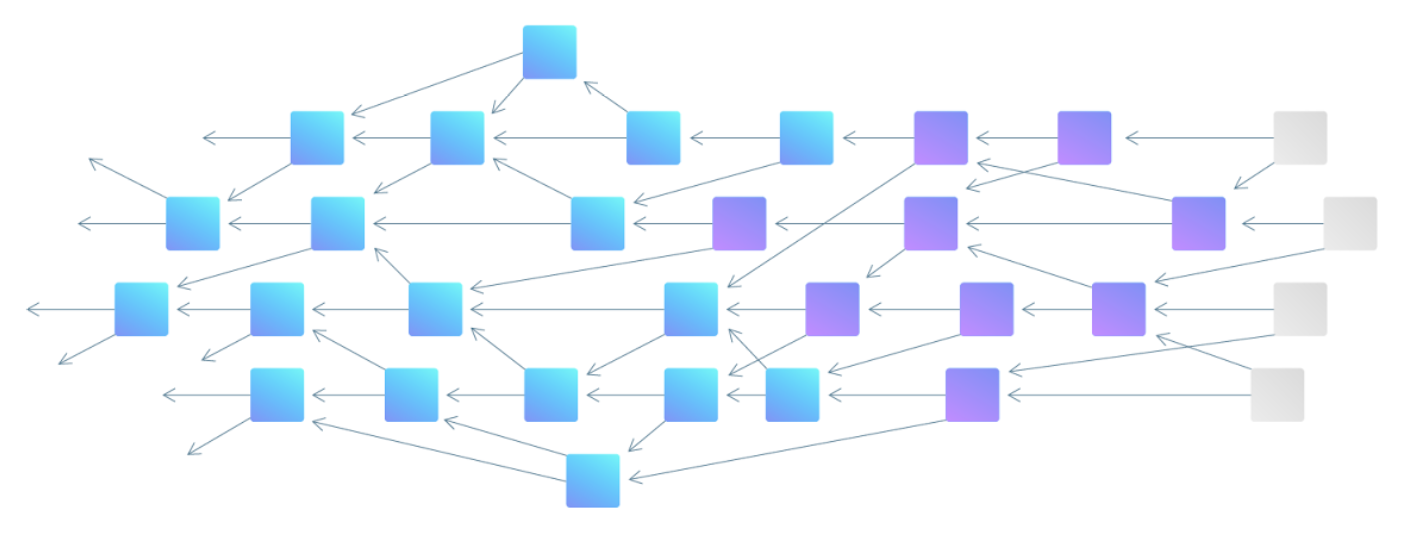
\includegraphics[width=1\textwidth]{tangle}
    \caption{Visualization of the tangle \cite{IOTA_Whitepaper}}
    \label{fig:tangle}
\end{figure}
The web of trust is a public-key authentication system originally built on PGP. A user can build confidence in their identity by having other users sign their public key \cite{Azouvi2017}. In an identity management system where we distinguish between Users and Service Providers, we can build on this idea. We can look at a scenario where a User has their identity verified and signed by visiting the governmental department issuing passports for their citizens. If the user wants proof that they also have a drivers license, and the issuing body (DMV, Statens Vegvesen, e.g.) trusts that department, they can link a drivers license to that identity based on the verified identity already in the ledger. This opens up for possibilities where the User can visit a small number of Identity Providers and establish a base identity, and then build upon that over the internet.
\newpage
Several academic papers propose Identity Management in blockchain applications, and the proposed implementation described in~\cite{Augot2017} provides functionality close to what is required in this system. They propose three types of actors; \textit{Identity Providers} (IP), \textit{Service Providers} (SP) and \textit{Users} (USR), and require three steps in their protocol; \textit{Setup Phase}, \textit{Enrollment Phase}, and \textit{Operational Phase}. In the \textit{Setup Phase}, the \textit{Identity Provider} chooses some set of attributes and makes them publicly available on the Bitcoin ledger. In the \textit{Enrollment Phase}, a \textit{User} brings proof of identity to the \textit{Identity Provider} (Physically or virtually, based on the policy of the \textit{Identity Provider}) that verifies all the attribute values of the claimed identity. This is finalized with a single transaction to the bitcoin ledger, that is considered a \textit{Authentication token}.  In the \textit{Operational Phase} the \textit{User} issues a transaction with the authentication token with outputs to both the \textit{Identity Provider} and back to itself for future transactions. The \textit{Service Provider} issues an Acknowledgement of the identity by sending output from the transaction to the \textit{Identity Provider}. The system is more complicated than described here, with possibilities for revocation and suggestions for storage outside of the blockchain by including the hash of the information in the \textit{OP\_RETURN} instead of the data itself. 

In \cite{Augot2017} the system relies on a Discrete Logarithm Representation (DLREP) proposed in \cite{Brands2000} to efficiently reveal selected parts of an identity to verifiers, while any other information remains hidden. The DLREP can be used to prove boolean functions about the identity, and will satisfy this systems requirement of privacy. 

In~\cite{Azouvi2017} the authors propose several solutions to register identities and attributes in a system built on public ledgers and compare them in terms of privacy, usability and integrity. Two of their solutions satisfy attribute integrity and privacy, and are named \textit{Multi-Casascius} and \textit{Mix-Network}. Both these solutions provide for passive verification, something the authors describes as the possibility to verify the identity only by looking at the public ledger - without the need for additional transactions or information from external sources.
